\documentclass[times, utf8, zavrsni, numeric]{fer}
\setlength{\parindent}{0em}
\tolerance=1
\emergencystretch=\maxdimen
\hyphenpenalty=10000
\hbadness=10000
\graphicspath{{../Slike/}}
\usepackage{hyperref}
\hypersetup{
	colorlinks=true,
	citecolor=black,
	linkcolor=black,
	urlcolor=cyan,
	pdflinkmargin=5pt
}

\begin{document}

% TODO: Navedite broj rada.
\thesisnumber{000}

\title{POVEZIVANJE VIRTUALNOG I STVARNOG OSVJETLJENJA KORIŠTENJEM UNREAL SUSTAVA}

\author{Bernard Bačani}

\maketitle

% Ispis stranice s napomenom o umetanju izvornika rada. Uklonite naredbu \izvornik ako želite izbaciti tu stranicu.
\izvornik

% Dodavanje zahvale ili prazne stranice. Ako ne želite dodati zahvalu, naredbu ostavite radi prazne stranice.
\zahvala{Zahvaljujem se Tiboru Jakovecu što je svaki dan išao sa mnom u menzu i svaki dan kasnio.}

\tableofcontents

\chapter{Uvod}

\chapter{Virtualna produkcija}
Filmska produkcija je izuzetno kompleksan proces koji je tipično linearan te se sastoji od razvoja, pretprodukcije, produkcije i postprodukcije (slika \ref{fig:slika 2-1}). Problem tradicionalne produkcije je izoliranost sudionika u pojedinoj fazi i neprilagodljivost promjenama na samom setu. Konačna verzija scene ne zna se do samog kraja produkcije, što uvelike otežava cijeli proces snimanja.\newline

\begin{figure}[htp]
	\centering
	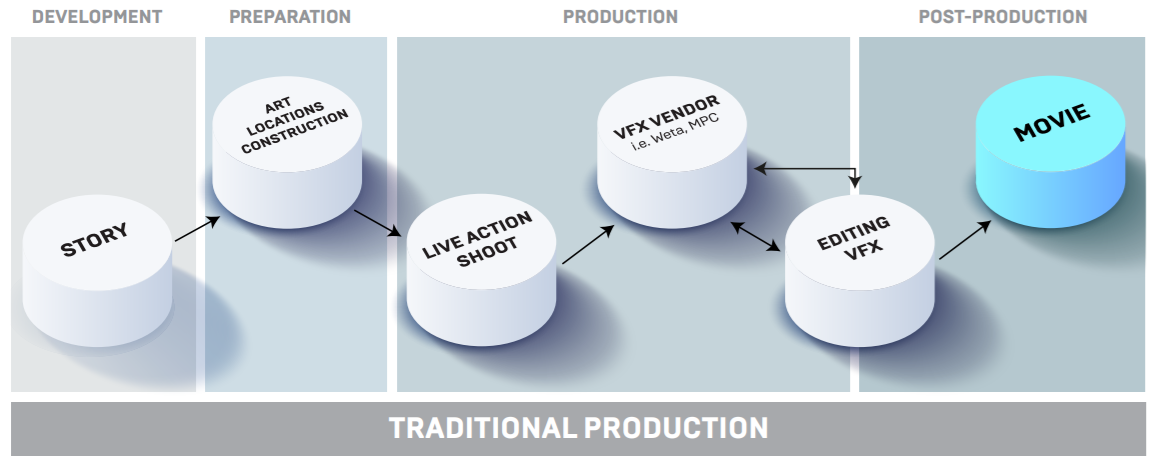
\includegraphics[width=\linewidth]{slika 2-1.png}
	\caption{Tradicionalna produkcija \cite{vpguide1}}
	\label{fig:slika 2-1}
\end{figure}

Virtualna produkcija je metoda slična agilnom razvoju, gdje se korištenjem pogonskog sklopa igara (engl. \emph{game engine}) prati kretnja kamere u stvarnom vremenu te se pozadinski sadržaj prikazuje na LED ekranu. Za razliku od tradicionalne, virtualna produkcija uvodi fleksibilnost u snimanje, omogućujući promjenu priče ili bilo kojeg dijela seta uz prisutnost cijelog tima, čime se štedi na vremenu i resursima (slika \ref{fig:slika 2-2}).

\begin{figure}[htp]
	\centering
	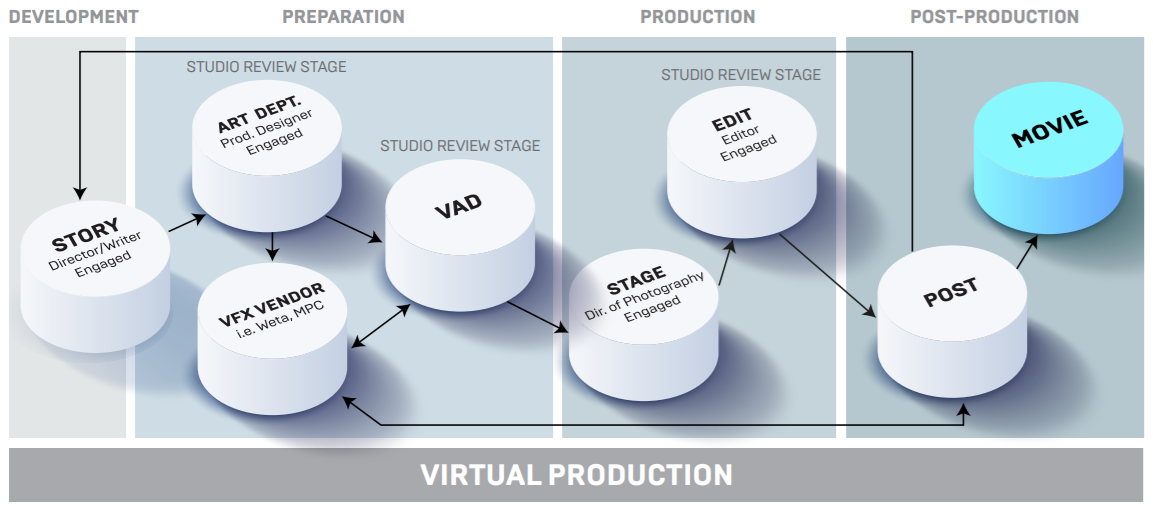
\includegraphics[width=\linewidth]{slika 2-2.png}
	\caption{Virtualna produkcija \cite{vpguide1}}
	\label{fig:slika 2-2}
\end{figure}

\section{Slučajevi upotrebe}
Vizualizacija je vjerojatno najčešći oblik upotrebe virtualne produkcije, a posebice predvizualizacija, koja u novoj paradigmi pruža prvi uvid u ideje i sredstva koja će se koristiti kroz produkciju \cite{vpguide2}. Poznata uporaba ove tehnike je u seriji \emph{The Mandalorian} (2019.-) gdje je virtualna produkcija bila korištena u snimanju više od pola cijele prve sezone (slika \ref{fig:slika 2-3}).\newline

Osim u filmovima i serijama može se koristiti u predvizualizaciji raznih javnih događaja poput koncerata. Primjerice, tvrtka Moment Factory je u 2021. godini objavila projekt \emph{DMX Previs}, digitalni svjetlosni šou (engl. \emph{light show}) napravljen koristeći DMX dodatak (engl. \emph{plugin}) u Unreal Engineu (slika \ref{fig:slika 2-4}) koji je sličan primjeru iz stvarnog života te ga se može i upravljati upravljačkom konzolom za osvjetljenje.\newline

Također, virtualna produkcija koristi se za hvatanje pokreta (engl. \emph{motion capture}) - praćenja pokreta objekata ili glumaca za animaciju digitalnih modela i kod vizualnih efekata u kameri (engl. \emph{in-camera visual effects}, skraćeno in-camera VFX).

\begin{figure}[htp]
	\centering
	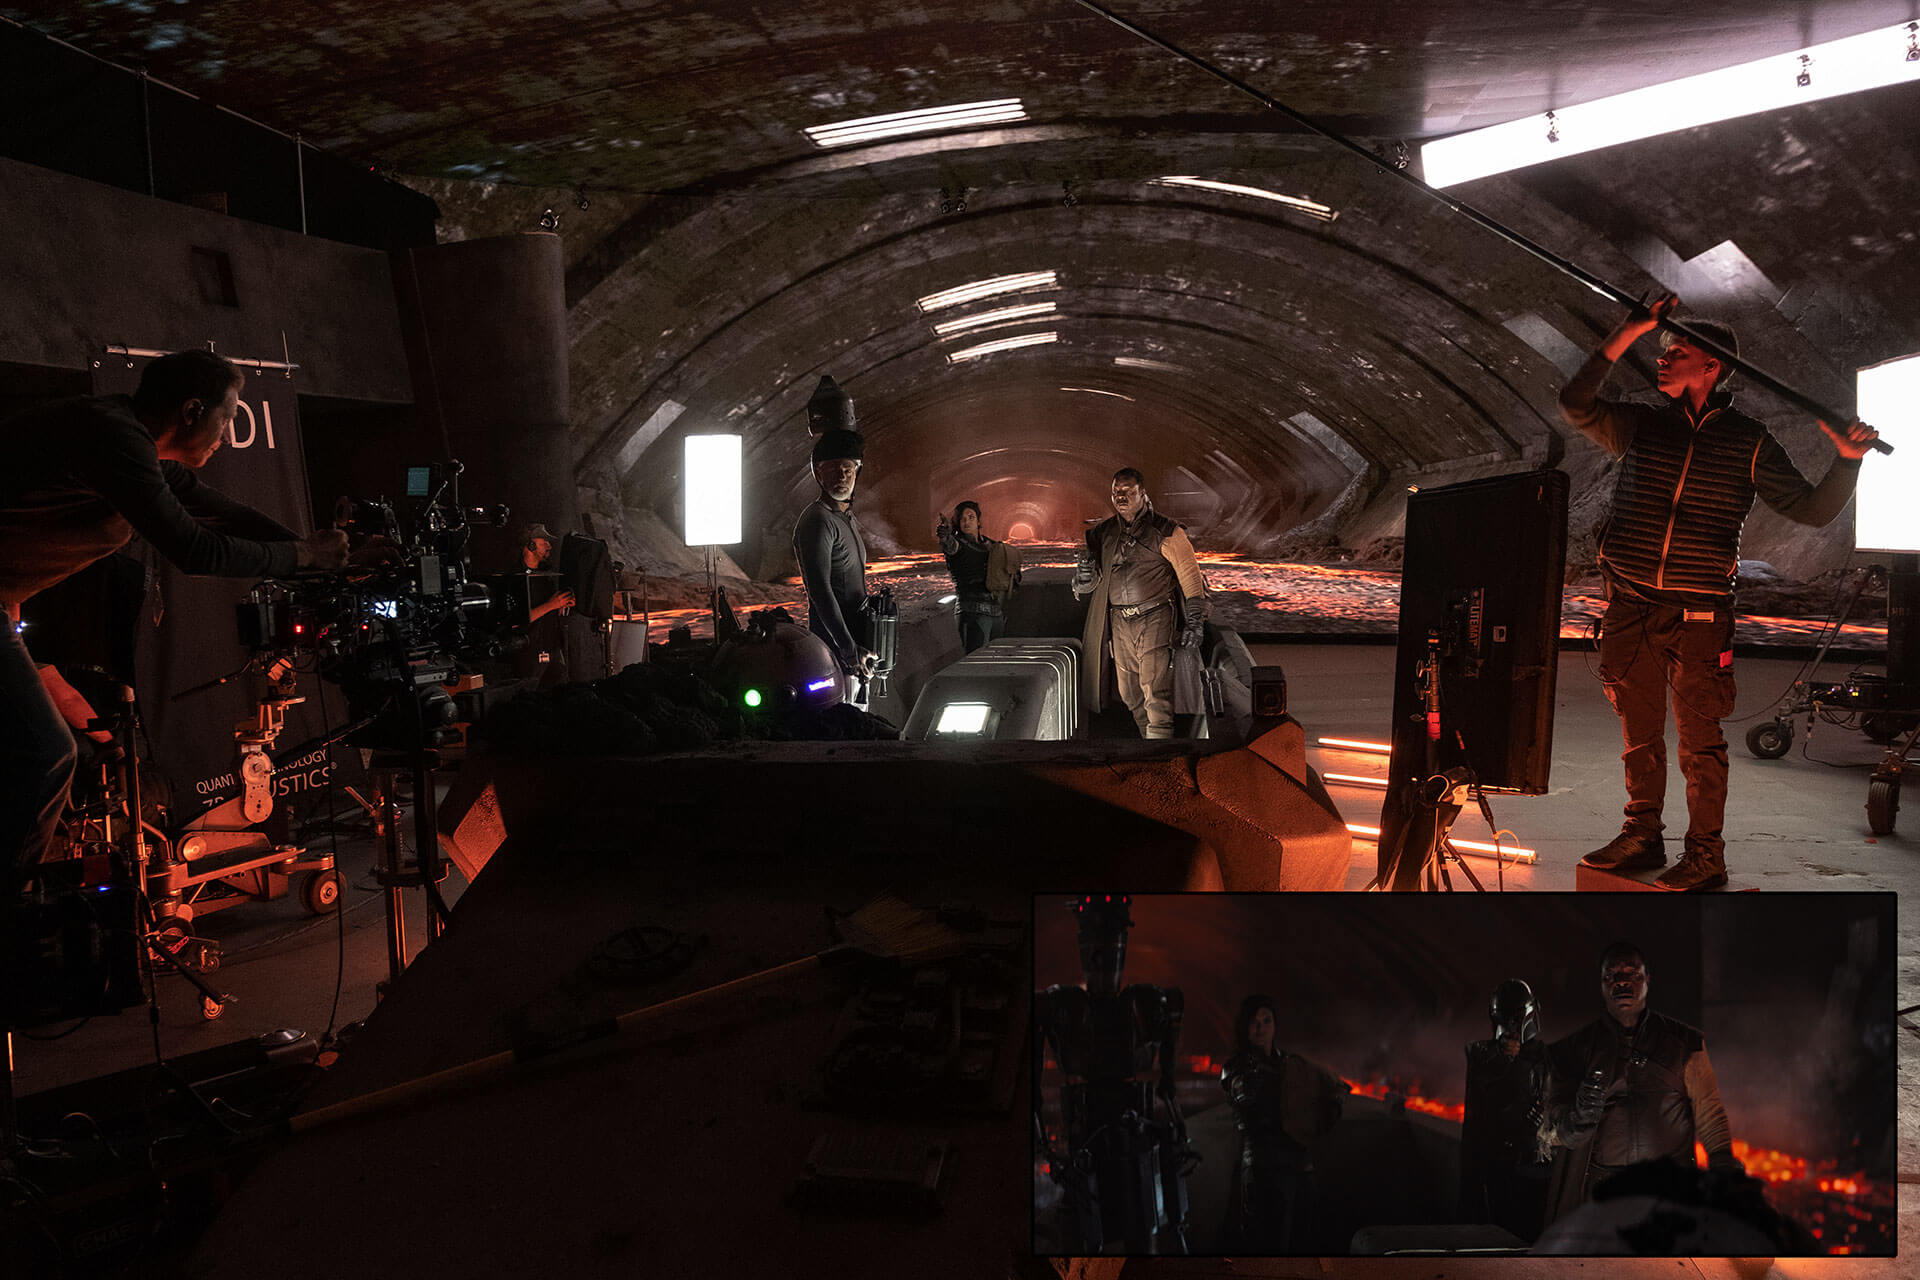
\includegraphics[width=\linewidth]{slika 2-3.png}
	\caption{Set u seriji \emph{The Mandalorian} \cite{mandalorian}}
	\label{fig:slika 2-3}
\end{figure}

\begin{figure}[htp]
	\centering
	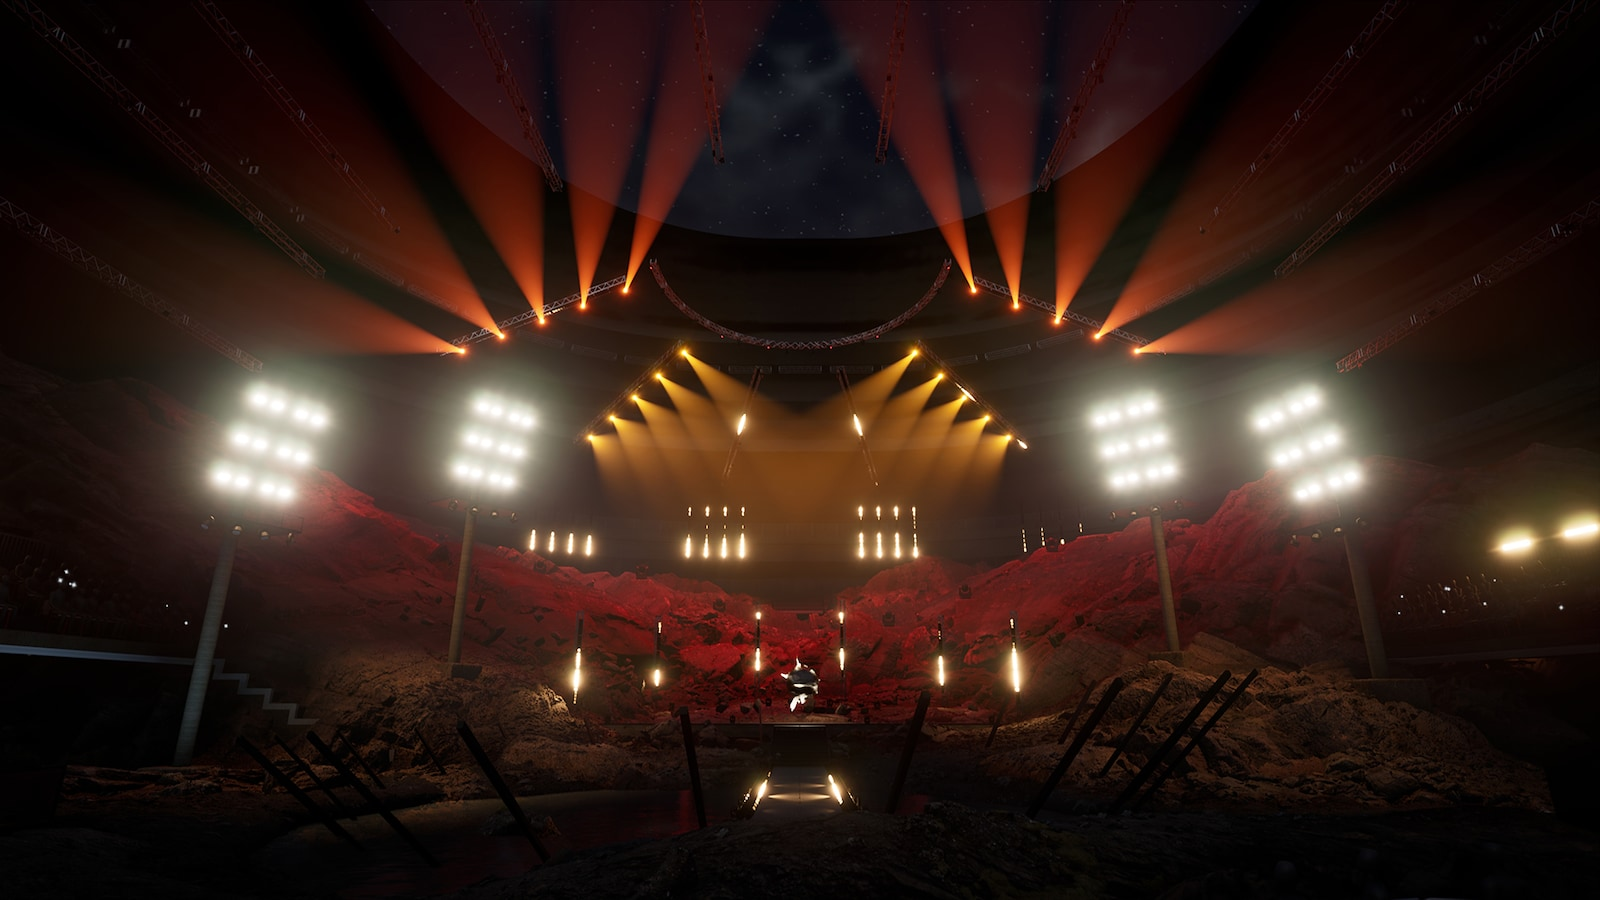
\includegraphics[width=\linewidth]{slika 2-4.png}
	\caption{Svjetlosni šou \emph{DMX Previs} \cite{dmx_previs}}
	\label{fig:slika 2-4}
\end{figure}

\pagebreak

\section{Opis prototipa}
Prototip za snimanje virtualne produkcije se sastoji od HTC Vive sustava sa dvije bazne stanice i HTC Vive Trackera nalijepljenog na kameru te LED ekrana računala. Kretanjem kamere HTC Vive Tracker detektira pokrete te se oni šalju iz stvarnog svijeta u virtualni svijet napravljen u Unreal Engineu, što rezultira promjenom virtualne kamere i scene prikazane na LED ekranu.\newline

Bazne stanice su postavljene na zamišljenu dijagonalu prostora gdje se obavlja snimanje te su priključeni na izvor struje, a HTC Vive Tracker je bežično spojen putem USB adaptera kako bi se dobila sloboda kretanja kamere. Navedeno sklopovlje je povezano sa računalom pomoću SteamVR aplikacije. \cite{vp}

\chapter{Upravljanje osvjetljenjem}
Za upravljanje osvjetljenjem u industriji se koristi konzola za upravljanje rasvjetom, elektronički uređaj koji komunicira sa svjetlima, prigušivačima i ostalim specijalnim efektima putem protokola upravljanja. Osim komuniciranja direktno, neke konzole mogu komunicirati s uređajima putem mreže pomoću mrežnih protokola.

\section{DMX}
Digital Multiplex (skraćeno DMX) je standardni digitalni komunikacijski protokol koji se uobičajeno koristi za upravljanje svjetlima i svjetlosnim efektima dajući im naredbe poput promjene boje, pozicije i intenziteta. Izvorno namijenjen kao standardna metoda za kontrolu prigušivača svjetlosti, brzo je proširio svoju namjenu na kontrolu ostalih uređaja, poput vatrometa, lasera, mikrokontrolera, inteligentna svjetla, uređaja za maglu itd.\newline

DMX možemo gledati kao paket digitalnih informacija koji se šalju s izvora na odredište pri čemu svaki paket sadrži polje od 512 bajtova čije su vrijednosti između 0 i 255 (slika \ref{fig:slika 3-1}).

\begin{figure}[htp]
	\centering
	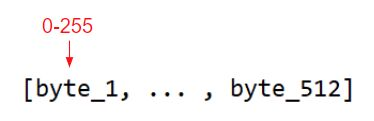
\includegraphics[width=\linewidth]{slika 3-1.png}
	\caption{DMX paket \cite{dmx_overview}}
	\label{fig:slika 3-1}
\end{figure}

\subsection{Kontroleri}
DMX kontroleri (engl. \emph{controllers}) djeluju kao izvor DMX paketa te šalju podatke do jednog ili više povezanih uređaja. Postoje dva oblika DMX kontrolera, USB/mrežno sučelje koje pretvara USB signale ili IP pakete u DMX te standardna DMX konzola koja omogućuje ručno aktiviranje slanja DMX paketa. Konzole također mogu imati podršku za komunikaciju preko mreže.

\subsection{Rasvjetni uređaji}
DMX rasvjetni uređaji (engl. \emph{fixtures}) su uređaji koji primaju DMX pakete te na temelju primljenih podataka obavljaju određenu naredbu. Naredbe mogu biti razne, obično uključivanje/isključivanje, pojačavanje/smanjivanje intenziteta, promjena boje te rotacija za neki kut.\newline

Svaki rasvjetni uređaj ima niz atributa koji su unaprijed definirani na hardverskoj razini te su organizirani u grupe koje zovemo odama (engl. \emph{odes}). Često uređaji imaju više načina rada (engl. \emph{mode}) kako bi korisnici mogli odabrati samo one funkcije koje im zaista trebaju te time pojednostavili upravljanje. Npr. ako neki uređaj ima ugrađenih 8 funkcija, a način rada mu se postavi na 4 kanalni, tada će samo prve 4 funkcije biti dostupne.\newline

Svemir (engl. \emph{universe}) u DMX-u predstavlja niz spojenih rasvjetnih uređaja koje čitaju iste podatke (pakete). Svaki svemir sadrži 512 adresa te se na jedan svemir može spojiti najviše 512 rasvjetnih uređaja (uz pretpostavku da su svi uređaji 1 kanalni). Dakle, rasvjetni uređaj će zauzimati onoliko adresa u svemiru koliko atributa ima u trenutnom načinu rada (4 kanalni način rada = 4 adrese).

\subsection{Komunikacija signala}
Svaki kontroler je zadužen za jedan ili više svemira te u svakom svemiru se nalazi nekoliko rasvjetnih uređaja. Kada kontroler šalje DMX paket, locira svemir kojemu ga treba poslati te šalje isti paket svakom rasvjetnom uređaju u tom svemiru. Paket se šalje slijedno, prvi uređaj pročita podatke u paketu te šalje paket dalje sljedećem. Kako bi uređaj pravilno primio podatke koji se odnose na njega, treba slušati odgovarajuće podatke u paketu, zbog čega je uvedeno adresiranje.\newline

Adresiranje (engl. \emph{fixture patching}) svakom rasvjetnom uređaju dodjeljuje specifičnu početnu adresu u svemiru, čime rasvjetni uređaj tada zauzima raspon adresa od početne adrese do početne adrese plus koliko je atributa u trenutnom načinu rada (slika \ref{fig:slika 3-2}).

\begin{figure}[htp]
	\centering
	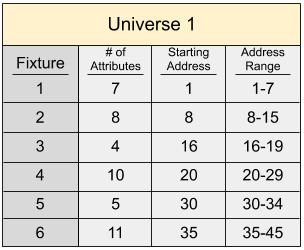
\includegraphics[width=\linewidth]{slika 3-2.png}
	\caption{Adresiranje \cite{dmx_overview}}
	\label{fig:slika 3-2}
\end{figure}

Prema primjeru na slici, kada se pošalje DMX paket, rasvjetni uređaj 4 će od 512 adresa u paketu slušati samo one na adresama 20-29, a ostale će zanemariti.\newline

Većinu vremena atributu će biti dovoljan opseg unosa od jednog bajta (0-255), ali ako želimo veću kontrolu te jedan bajt nije dovoljan, atribut može zauzeti više adresa u svemiru. Primjerice, atribut koji zauzima dvije adrese može poprimiti vrijednosti u rasponu 0-65,536. Ostali primjeri:

\begin{enumerate}
	\item 8-bitni atribut - Min: 0, Max: 255 - zauzima 1 adresu
	\item 16-bitni atribut - Min: 0, Max: 65,536 - zauzima 2 adrese
	\item 24-bitni atribut - Min: 0, Max: 16,777,215  - zauzima 3 adrese
	\item 32-bitni atribut - Min: 0, Max: 4,294,967,296  - zauzima 4 adrese
\end{enumerate}

\section{Mrežni protokoli}
Porastom kompleksnosti i broja uređaja korištenih u predstavama pojavila se potreba za lakšim i bržim adresiranjem i upravljanjem rasvjetnim uređajima. Napretkom komunikacijskih tehnologija razvijeni su ethernet protokoli koji omogućuju prijenos više DMX svemira putem Cat5 kabla. Unreal Engine podržava dva ethernet protokola, Art-Net i sACN.

\subsection{Art-Net}
Art-Net je ethernet protokol temeljen na paketu protokola TCP/IP te se koristi za prijenos velikog broja DMX paketa putem UDP protokola. Najnovija revizija je Art-Net 4 i podržava prijenos 32,768 svemira (teoretski, stvarni broj ovisi o fizičkom sloju mreže i metodi prijenosa) i preko 1000 DMX priključaka (engl. \emph{ports}), gdje je adresa priključka svakog svemira kodirana kao 15-bitni broj (slika \ref{fig:slika 3-3}).

\begin{figure}[htp]
	\centering
	\includegraphics[width=\linewidth]{slika 3-3.png}
	\caption{Adresa priključka svakog DMX svemira \cite{art-net}}
	\label{fig:slika 3-3}
\end{figure}

Podmreža (engl. \emph{Sub-Net}) je grupa od 16 uzastopnih svemira, a mreža (engl. \emph{Net}) je grupa od 16 uzastopnih podmreža ili 256 uzastopnih svemira.\newline

Kod prvog spajanja mreže, kontroleri ne znaju broj uređaja u mreži ni njihove IP adrese te se za njihovo otkrivanje koristi \emph{broadcast} adresa - kontroler pošalje \emph{ArtPoll} paket na IP adresu 2.255.255.255 na UDP priključku 0x1936. \emph{ArtPoll} paket šalje samo kontroler, a odgovor \emph{ArtPollReply} šalju i kontroleri i uređaji. Maksimalno vrijeme čekanja između slanja \emph{ArtPoll} paketa i primanja \emph{ArtPollReply} paketa je 3 sekunde. Kontroler koji je poslao \emph{ArtPoll} paket bi također trebao odgovoriti na svoju poruku sa \emph{ArtPollReply}, čime se osigurava da bilo koji drugi kontroleri koji slušaju na mreži detektiraju sve uređaje bez potrebe da svaki spojeni kontroler šalje \emph{ArtPoll} paket. Svi kontroleri moraju poslati \emph{ArtPoll} svakih 2.5 do 3 sekunde, čime se lako otkriva prekid veze.\newline

Za prijenos DMX podataka koristi se \emph{unicast} ili \emph{broadcast} adresa te se šalje \emph{ArtDmx} podatkovni paket (slika \ref{fig:slika 3-4}).

\begin{figure}[htp]
	\centering
	\includegraphics[width=\linewidth]{slika 3-4.png}
	\caption{Prijenos DMX paketa \cite{streaming_packets}}
	\label{fig:slika 3-4}
\end{figure}

Iako se za slanje \emph{ArtDmx} paketa može koristiti broadcast adresa, u velikom sustavu dolazi do ogromnog opterećenja obrade podataka te se koristi \emph{unicast} adresa. Kako bi se mogla koristiti \emph{unicast} adresa, kontroleri trebaju znati  koji uređaji slušaju na određenom priključniku, što se ostvaruje preplatom (engl. \emph{subscription}). Pretplata se odvija na sljedeći način: \cite{subscription}

\begin{enumerate}
	\item Kontroler na \emph{broadcast} adresu šalje \emph{ArtPoll} svakih 2.5 do 3 sekunde.
	\item Kontroler analizira sve \emph{ArtPollReply} pakete i sastavlja popis do 8 mogućih priključnih adresa i pridružene IP adrese za svaki uređaj koji odgovori (pretplatnici).
	\item Kontroler koristi ovaj popis za izračunavanje IP adrese koju bi trebao koristiti za slanje \emph{ArtDmx} paketa na \emph{unicast} adresu.
\end{enumerate}

\emph{ArtSync} paket koristi se za sinkronizaciju slanja \emph{ArtDmx} paketa. Sinkronizacija se odvija tako da kontroler na \emph{unicast} adrese svemira šalje \emph{ArtDmx} pakete, a zatim na \emph{broadcast} adresu pošalje jedan \emph{ArtSync} paket koji signalizira da je zadnji \emph{ArtDmx} paket stigao na odredište.

\pagebreak

\subsection{sACN}
Arhitektura strujanja za upravljačke mreže (engl. \emph{Streaming Architecture for Control Networks}, skraćeno sACN) je standardni protokol razvijen za efikasni prijenos DMX svemira preko mreže. Konceptualno je veoma usporediv s Art-Netom te se sastoji od podatkovni paket (\emph{E1.31 Data Packet}) za prijenos DMX podataka, paket otkrivanja (\emph{E1.31 Universe Discovery Packet}) za praćenje prometa i sinkronizacijski paket (\emph{E1.31 Synchronization Packet}). Za razliku od Art-Neta, podržava prijenos do 63,999 svemira i \emph{multicast} adrese, čime se mogu prenositi podaci bez prethodnog znanja topologije mreže \cite{sACN}.

\section{GDTF}
\emph{General Device Type Format} (skraćeno GDTF) protokol je otvoreni standard razvijen kako bi se olakšala primjena novih rasvjetnih uređaja (slika \ref{fig:slika 3-5}). GDTF datoteka je otvorenog formata te se sastoji od XML datoteke koja sadrži informacije o pojedinom uređaju poput geometrije, atributa, načina rada i pretpostavljenih vrijednosti \cite{dmx_gdtf}. Baza podataka svih dostupnih GDTF datoteka je besplatna \cite{GDTF}.\\

\begin{figure}[htp]
	\centering
	\includegraphics[width=\linewidth]{slika 3-5.png}
	\caption{GDTF \cite{GDTF}}
	\label{fig:slika 3-5}
\end{figure}

\chapter{Model rješenja}
Upravljačka konzola za osvjetljenje je uređaj kojim se upravlja svjetlosnim i drugim uređajima putem upravljačkog protokola. Zbog povećane količine uređaja na pozornici, osim komuniciranja direktno ili preko USB-a, neke konzole također mogu komunicirati putem mreže kako bi se olakšala kontrola nad složenim sustavima. Za ovaj rad korišten je simulator konzole koji šalje podatke preko ethernet protokola.\newline

Svjetlosni efekti korišteni u simulaciji su nalik na one u javnima događajima, poput koncerata gdje se koriste primjerice reflektori, laseri, dimni efekti i drugo.
Zatim, simulacija se integrira s postojećim sustavom za detekciju položaja kamere u kojem se pomoću stvarne kamere upravlja virtualnom kamerom u stvarnom vremenu.

\section{Simulacija osvjetljenja}
Simulacija je zamišljena kao predvizualizacija mini pozornice u kazalištu. Pozornica sadrži nekoliko reflektora, statičnih svjetala i lasera. Svjetlosnim uređajima se upravlja simulatorom konzole te se svjetla pale i gase, mijenja im se pozicija, pojačava ili smanjuje intenzitet i slično. Promatra se slanje naredbi korištenjem konzole u stvarnom vremenu te unaprijed programiran skup naredbi koji se izvodi u sekvenceru. Simulacija je uspješna ako je dobiven rezultat sličan korištenju prave konzole te je utjecaj kašnjenja minimalan.

\section{Integracija s prototipom}
Povezivanje s prototipom ostvaruje se korištenjem stvarne kamere, sustava za virtualnu stvarnost i LED zaslona. Kako se simulacija izvodi, kretanjem stvarne kamere mapiraju se pokreti u virtualnu kameru te se time krećemo po pozornici. Ispred LED zaslona stavljaju se objekti u stvarnom životu te se snima smješten objekt u virtualnoj sceni. Integracija je uspješna ako se dobije dojam da se objekt stvarno nalazi na pozornici, a simulirana svjetlost nalikuje stvarnoj svjetlosti.

\chapter{Korištene tehnologije}
\textbf{Unreal Engine} \cite{Unreal_Engine} je pogonski sklop igre (engl. \emph{game engine}) prvenstveno namijenjen za razvoj digitalnih igara za PC. Može se koristiti za izradu dvodimenzionalnih i trodimenzionalnih igara, aplikacija za virtualnu i proširenu stvarnost te za razvoj virtualnih setova korištenih u filmskoj industriji. Skripte se pišu programiranjem u jeziku C++ ili korištenjem vizualnog sustava skriptiranja \emph{Blueprints}. 
Za izradu i testiranje simulacije korišten je Unreal Engine 4.26.2.\newline

\textbf{MagicQ Software} \cite{MagicQ_Software} je programsko sučelje za vizualizaciju i kontrolu osvjetljenja do 256 svemira (64 svemira za PC verziju). Omogućuje slanje DMX paketa preko mreže do aplikacija na računalu korištenjem Art-Net, Pathport, sACN i drugih protokola. Korisničko sučelje i funkcionalnosti su jednake kao i na fizičkoj konzoli te je moguć međusobni prijenos podataka preko mreže ili USB-a. 
Za izradu i  testiranje simulacije korišten je MagicQ v1.8.9.0.\newline

\textbf{SteamVR} \cite{SteamVR} je alat za pokretanje VR sadržaja na sustavima za virtualnu stvarnost poput HTC Vive, Oculus Rift i drugi. Koristi \emph{Lighthouse} sustav, laserski sustav za praćenje položaja i orijentacije korisnika u stvarnom vremenu te \emph{Chaperone} sustav za postavljanje i pregled granica prostora u sobi kako bi se spriječilo kretanje izvan dosega senzora te zaletavanje u zidove i druge predmete.
Za testiranje simulacije korišten je SteamVR 1.16.10\newline

\textbf{HTC Vive} \cite{HTC_Vive} je sustav za virtualnu stvarnost koji omogućuje korisniku kretanje u 3D prostoru te interakciju sa okolinom korištenjem ručnih kontrolera. Osim \emph{headseta}, kontrolera i baznih stanica može se koristiti dodatak HTC Vive Tracker za praćenje pozicije predmeta na koji je pričvršćen preko \emph{Lighthouse} sustava.
Za testiranje simulacije korišten je HTC Vive Tracker, HTC Vive Tracker Dongle, HTC Vive Tracker Dongle Cradle i dvije bazne stanice.\newline

\textbf{DMX Template} \cite{dmx_template} je demo projekt u Unreal Engineu sa već omogućenim svim DMX dodacima te sadrži nacrte (engl. \emph{blueprints}) za DMX rasvjetne uređaje. Nacrti sadrže komponente koje su odgovorne za primanje DMX paketa. Projekt također sadrži tri mape sa unaprijed snimljenim ulaznim nizom DMX paketa.

\chapter{Izrada simulacije osvjetljenja}

\section{Postavljanje simulatora}
Slanje DMX paketa preko mreže ostvareno je pomoću \emph{ChamSys MagicQ} simulatora. Stvoren je novi šou u načinu programiranja \emph{Normal (live)} te kako bi se paketi mogli poslati lokalno na aplikacije na računalu, potrebno je otići u \emph{Setup} te u izborniku \emph{Network} postaviti opciju \emph{Send to Applications on this PC} na \emph{Yes}. Dodatno, u \emph{Setupu} u izborniku \emph{View DMX I/O} potrebno je omogućiti svemire kojima želimo upravljati postavljanjem opcije \emph{Status} na \emph{Enabled}. Za potrebe ovog rada omogućeni su svemiri 1 i 2. Ovdje se također mogu mijenjati ostale opcije poput imena svemira, protokola za prijenos paketa te način slanja paketa. Unreal Engine trenutno podržava samo Art-Net i sACN protokole te je ostavljena zadana vrijednost, odnosno Art-Net.\newline

Rasvjetne uređaje povezujemo u sustav u izborniku \emph{Patch}. Uređaj se dodaje odabirom \emph{Choose Head} čime se može izabrati uređaj iz postojeće kolekcije uređaja koji dolaze instalirani sa simulatorom ili se može napraviti vlastiti odabirom \emph{Edit Head} > \emph{New Head}. Za testno povezivanje odabran je uređaj \emph{Clay Paky Sharpy} u standardnom načinu rada (16-kanalni). Nakon što je odabran uređaj, klikne se na \emph{Patch It} te se upiše koliko uređaja će se spojiti. Pojavljuje se iskočni prozor sa opcijom umetanja uređaja u \emph{MagicQ} vizualizator, što se odbija jer se simulator koristi samo za slanje DMX paketa do Unreal sustava \cite{MagicQ_Manual}.

\section{Povezivanje s Unreal Engineom}
Napravljen je novi prazan (engl. \emph{Blank}) projekt te su uključeni dodaci (engl. \emph{plugins}) za DMX podršku, \emph{DMX Engine}, \emph{DMX Fixtures}, \emph{DMX Pixel Mapping} i \emph{DMX Protocol}. Dodatak \emph{DMX Fixtures} je trebao uvesti osnovne sheme, ali pošto nije uspio ručno je uvezena datoteka \emph{BP\_MovingHead.uasset} kopiranjem sa lokacije \path{C:\Program Files\Epic Games\UE_4.26\Engine\Plugins\VirtualProduction\DMX\DMXFixtures\Content\LightFixtures} u \emph{Content} direktorij našeg projekta.

Nakon toga, potrebno je kreirati \emph{DMX Library} odabirom \emph{Add/Import} > \emph{DMX} > \emph{DMX Library}. U izborniku \emph{Controllers} klikom na gumb \emph{New Controller} doda se novi DMX Controller te mu se uređuju svojstva (slika \ref{fig:slika 6-1}). \emph{Remote Universe Range Start} je postavljen na 0 jer \emph{Output Universe} u \emph{MagicQ} simulatoru počinje sa indeksom 0 \cite{MagicQ_Setup}.

\begin{figure}[htp]
	\centering
	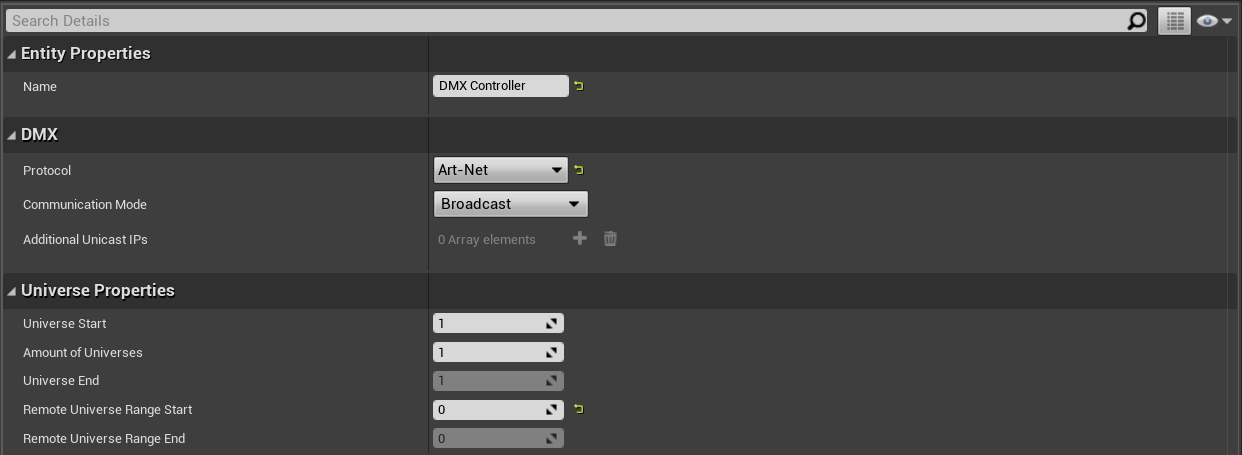
\includegraphics[width=\linewidth]{slika 6-1.png}
	\caption{Postavke kontrolera}
	\label{fig:slika 6-1}
\end{figure}

Zatim u izborniku \emph{Fixture Types} klikom na gumb \emph{New Fixture Type} doda se nova vrsta rasvjetnog uređaja. Postavke uređaja mogu se postaviti uvozom GDTF datoteke ili ručno. U \emph{Modes} i \emph{Mode Properties} pregledniku postavlja se način rada, a u \emph{Functions} i \emph{Function Properties} pregledniku postavljaju se funkcije uređaja (slika \ref{fig:slika 6-2}). Ako neka funkcija zauzima dva ili više kanala, \emph{Data Type} se postavi na odgovarajući broj bitova (jedan kanal zauzima jedan bajt).

\begin{figure}[htp]
	\centering
	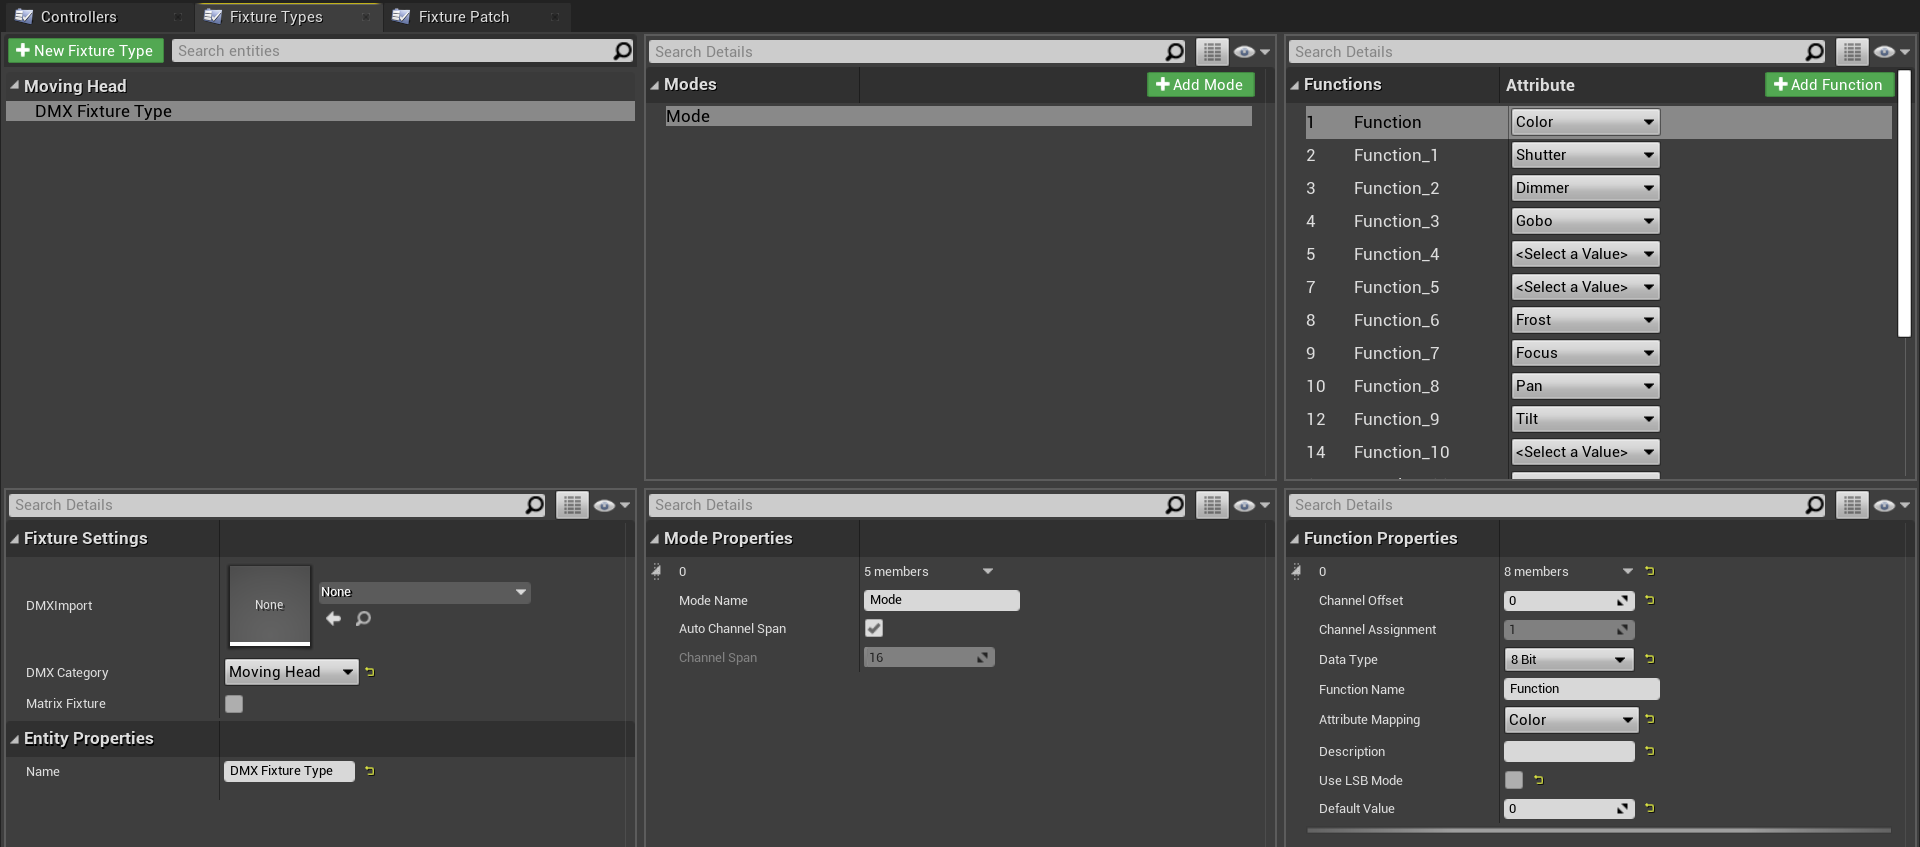
\includegraphics[width=\linewidth]{slika 6-2.png}
	\caption{Postavke uređaja}
	\label{fig:slika 6-2}
\end{figure}

Na kraju, potrebno je obaviti adresiranje u izborniku \emph{Fixture Patch}. Klikom na gumb \emph{Add Fixture} odabere se novokreirani uređaj te mu se postave svemir i adrese (slika \ref{fig:slika 6-3}).

\begin{figure}[htp]
	\centering
	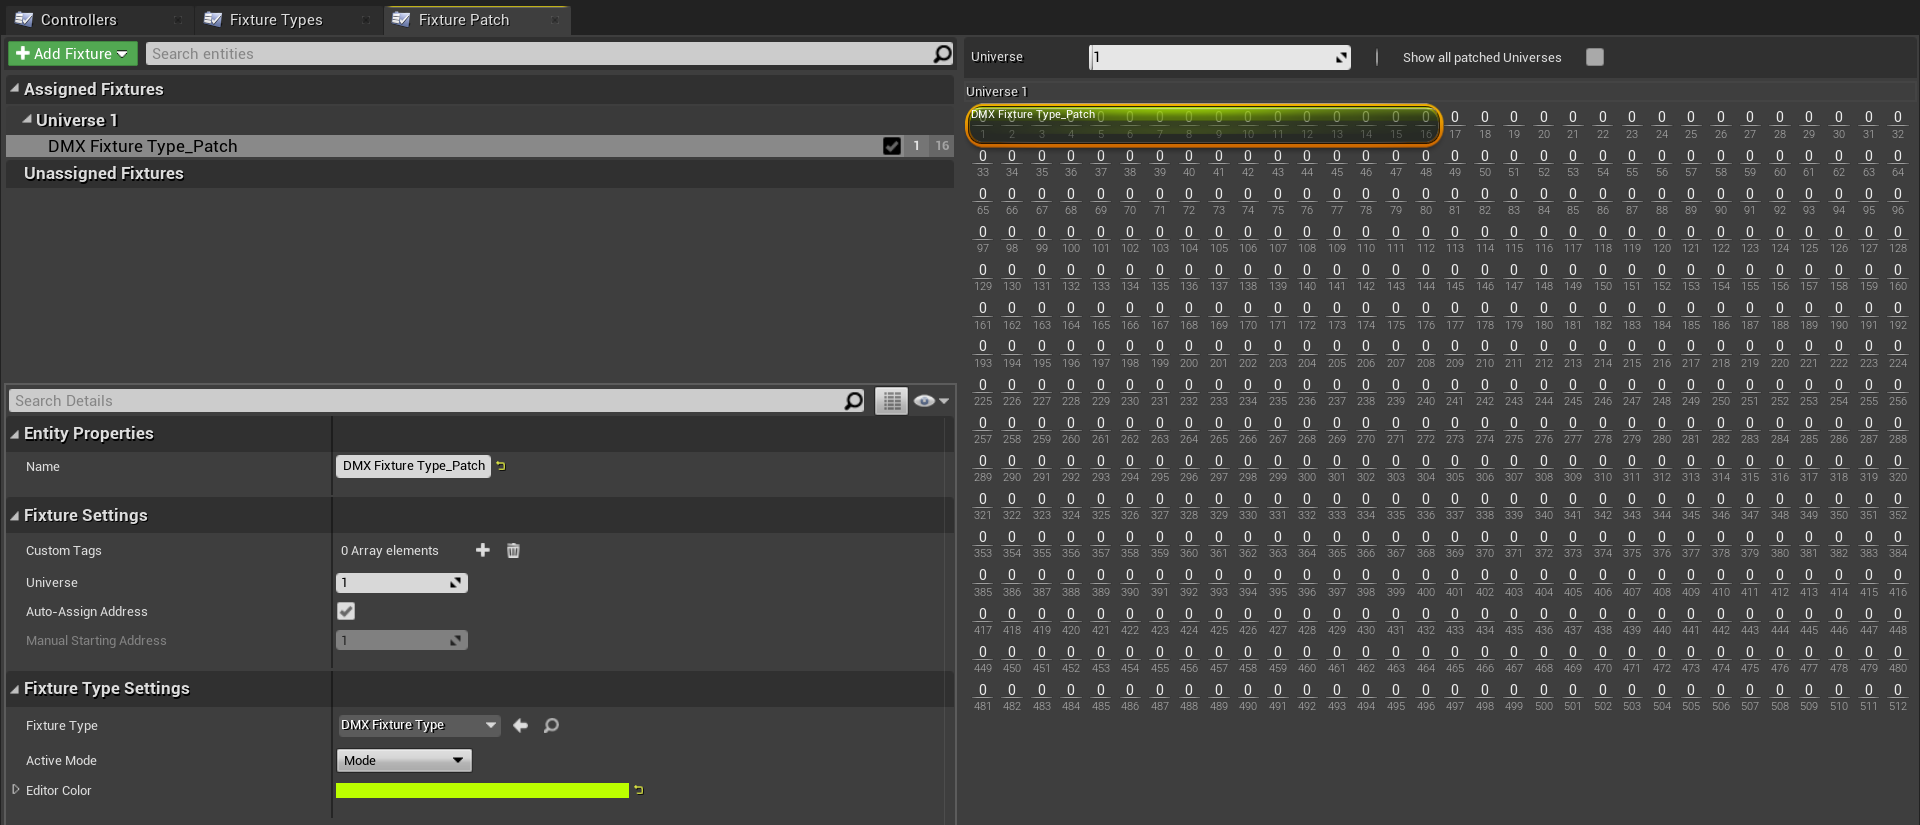
\includegraphics[width=\linewidth]{slika 6-3.png}
	\caption{Adresiranje uređaja}
	\label{fig:slika 6-3}
\end{figure}

Pregled svih dolaznih DMX paketa za pojedini svemir može se vidjeti u \emph{DMX Channel Monitoru} ili u \emph{DMX Activity Monitoru} \cite{dmx_quickstart}.\newline

Za testiranje je ubačen \emph{BP\_MovingHead} u scenu te mu je unutar \emph{Details} izbornika postavljen \emph{DMX Library} i \emph{Fixture Patch} (slika \ref{fig:slika 6-4}).

\begin{figure}[htp]
	\centering
	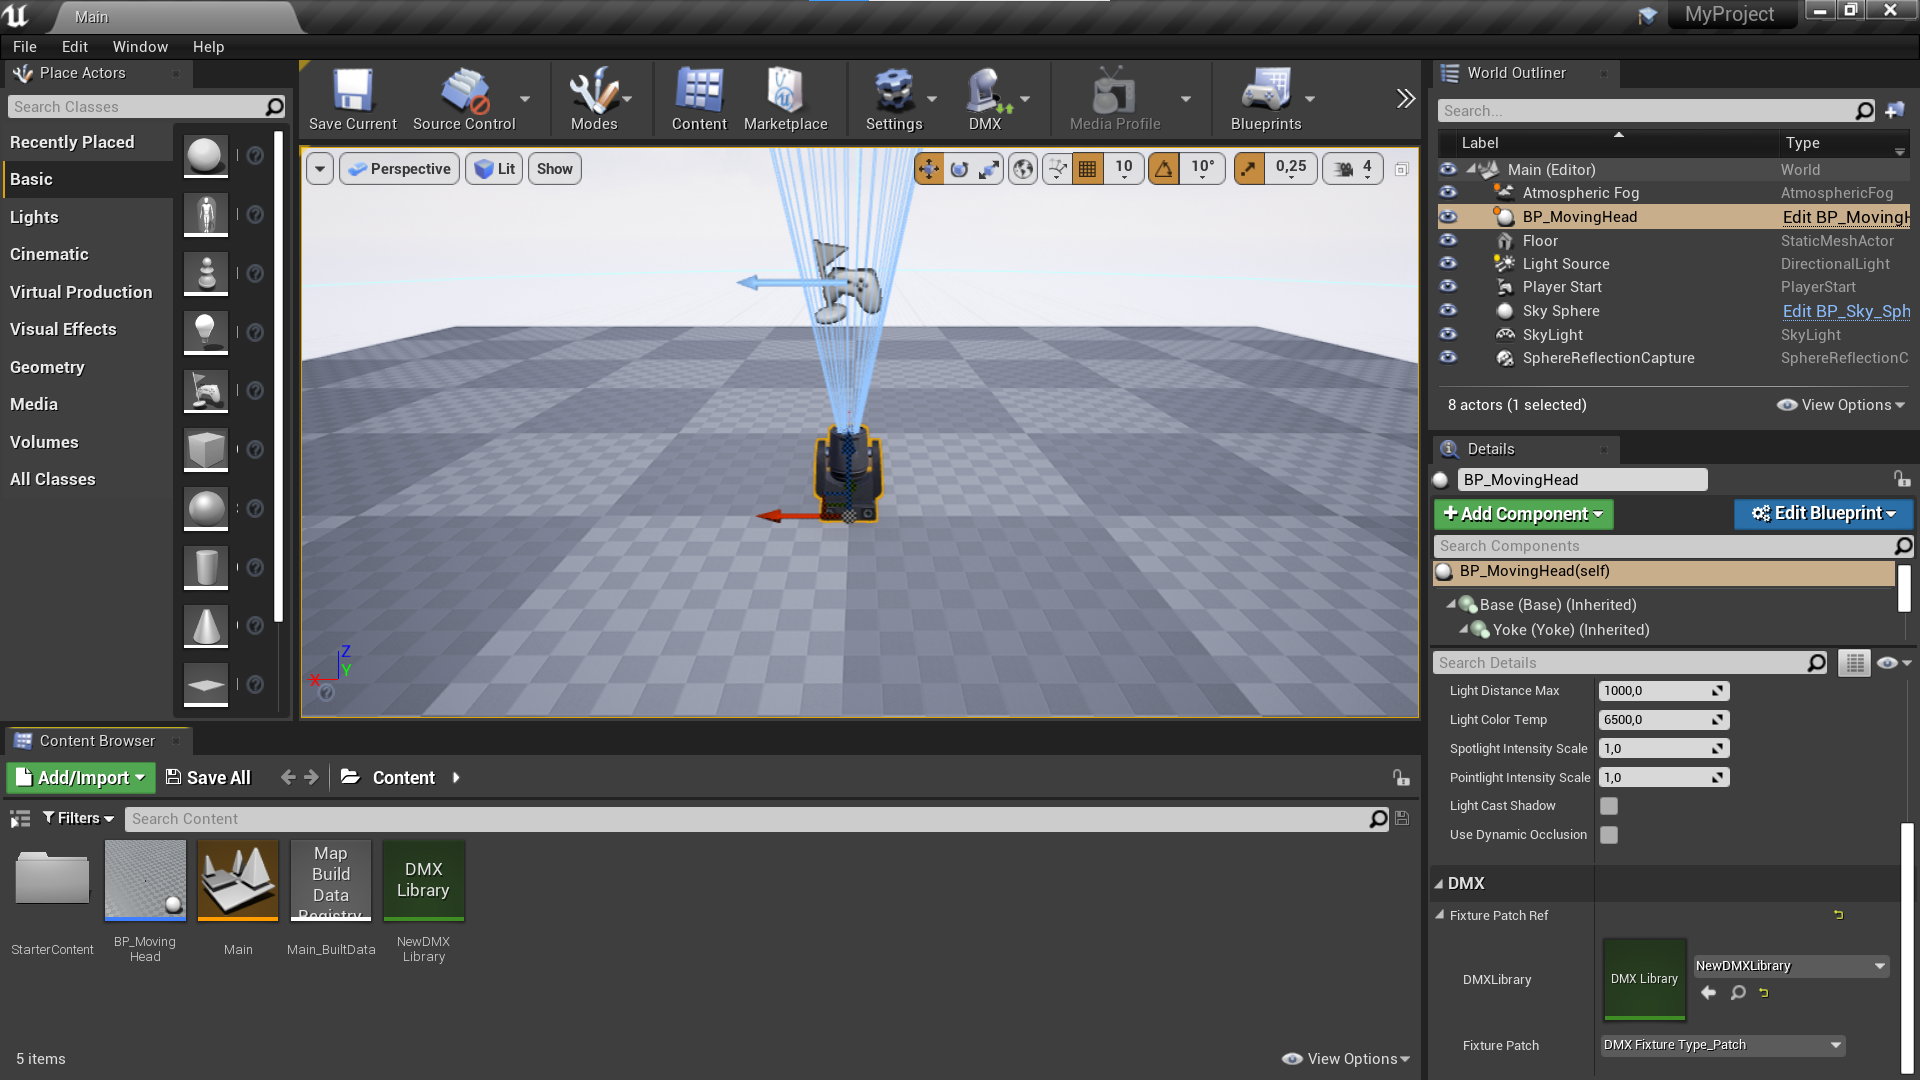
\includegraphics[width=\linewidth]{slika 6-4.png}
	\caption{Scena i DMX postavke pokretne glave}
	\label{fig:slika 6-4}
\end{figure}

Nakon pokretanja scene, korištenjem simulatora šalju se DMX paketi do Unreal Enginea što uzrokuje upravljanje pokretnom glavom (slike \ref{fig:slika 6-5} do \ref{fig:slika 6-8}).

\begin{figure}[htp]
	\centering
	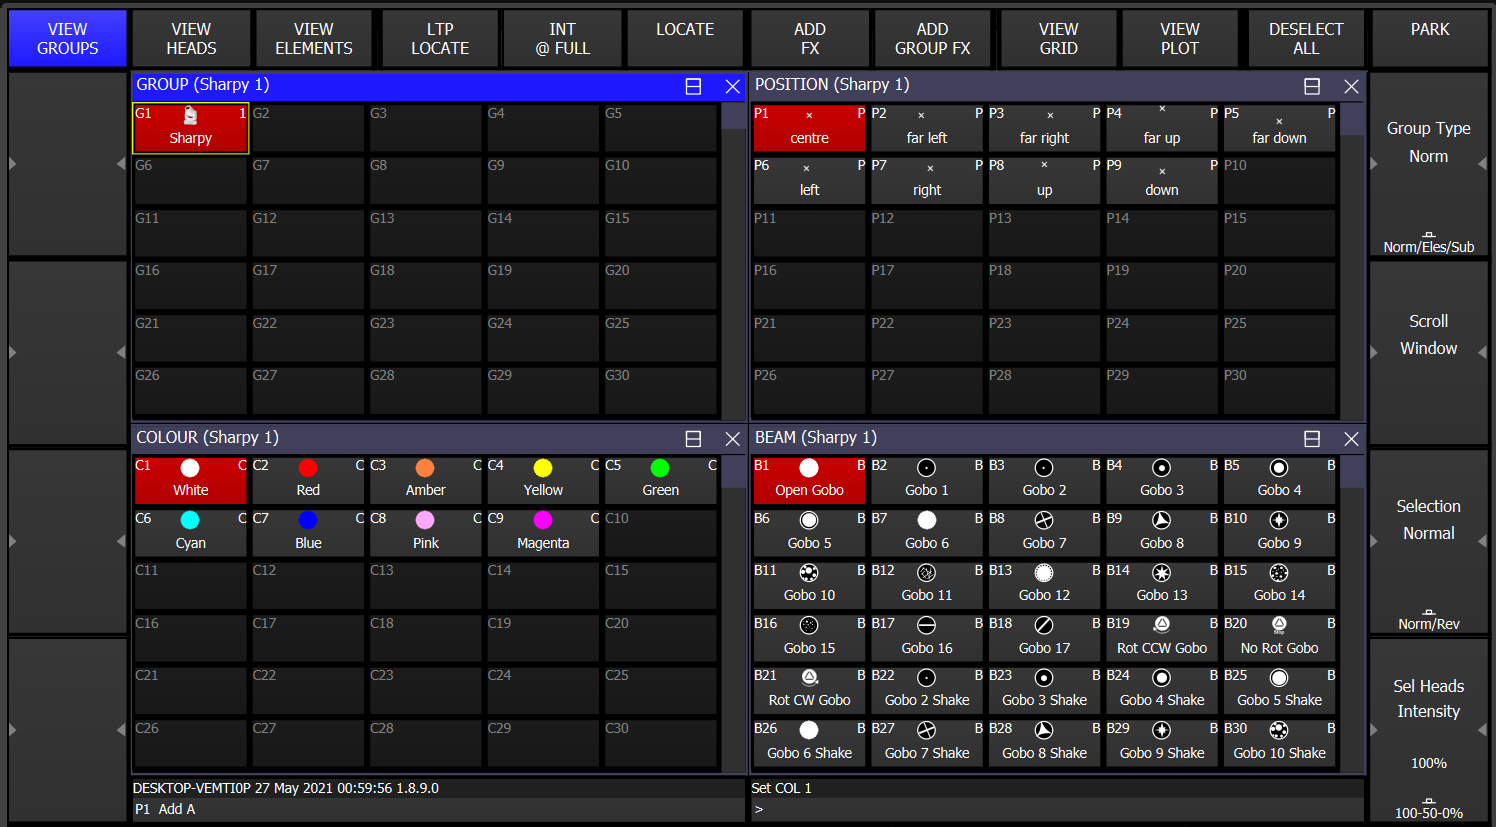
\includegraphics[width=\linewidth]{slika 6-5.png}
	\caption{Početno stanje simulatora}
	\label{fig:slika 6-5}
\end{figure}

\begin{figure}[htp]
	\centering
	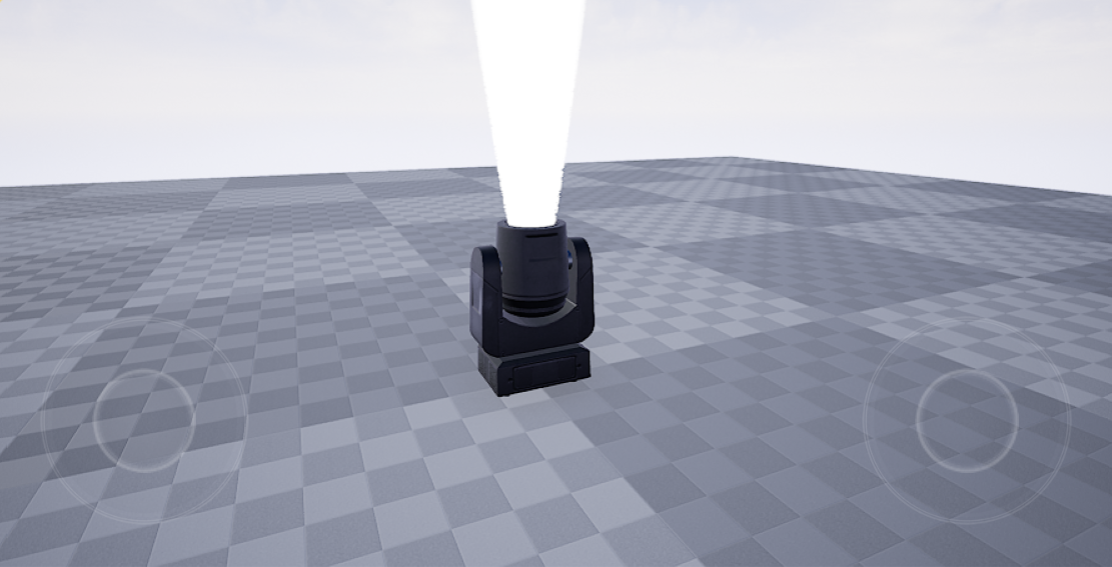
\includegraphics[width=\linewidth]{slika 6-6.png}
	\caption{Početno stanje pokretne glave}
	\label{fig:slika 6-6}
\end{figure}

\begin{figure}[htp]
	\centering
	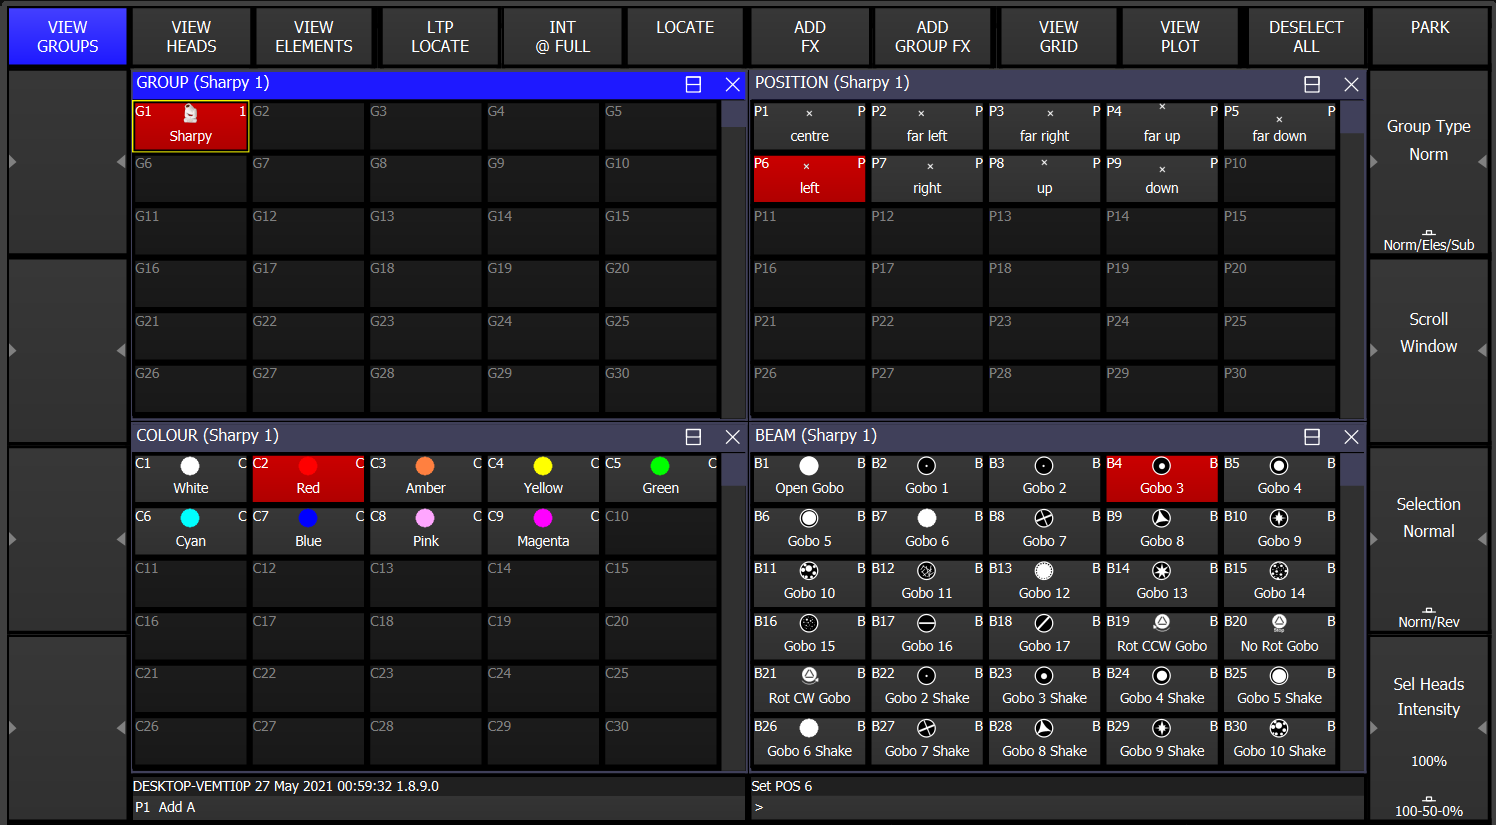
\includegraphics[width=\linewidth]{slika 6-7.png}
	\caption{Promjena pozicije, boje i zrake}
	\label{fig:slika 6-7}
\end{figure}

\begin{figure}[htp]
	\centering
	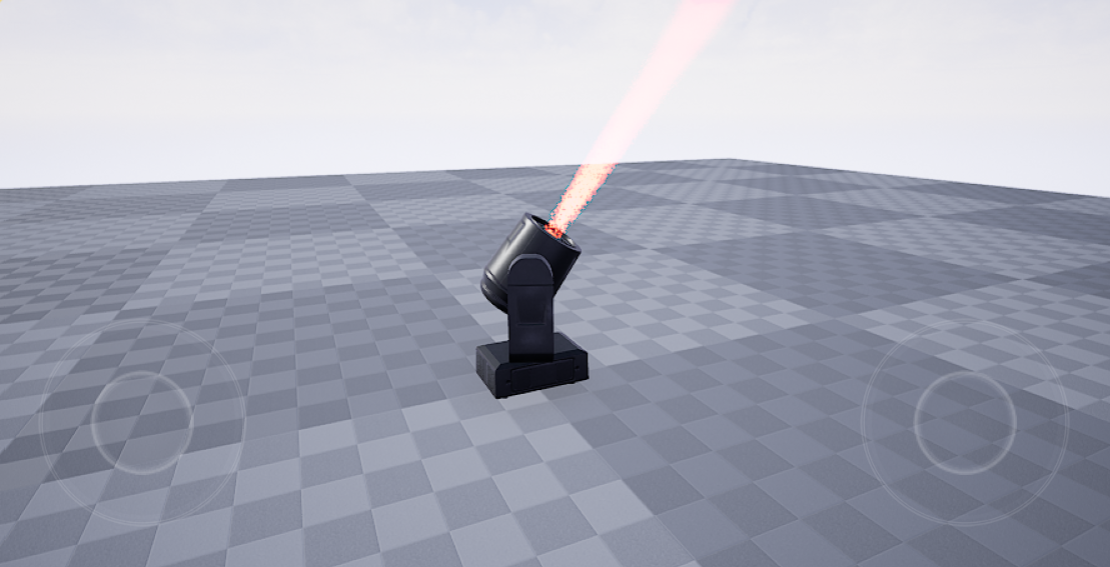
\includegraphics[width=\linewidth]{slika 6-8.png}
	\caption{Promjena stanja pokretne glave}
	\label{fig:slika 6-8}
\end{figure}

\section{Simulacija}
Za simulaciju je korišten \emph{DMX Template} koji već sadrži podešen cijeli \emph{DMX Library} i posložene rasvjetne uređaje u sceni. Potrebno je samo promijeniti \emph{Remote Universe Range Start} sa 1 u 0 kako bi se postigla kompatibilnost sa \emph{MagicQ} simulatorom.

\subsection{Upravljanje simulatorom}
U \emph{MagicQ} simulatoru za svaku vrstu rasvjetnog tijela u sceni stvori se nova glava (engl. \emph{Head}) te se dodijele jednake funkcije i početne vrijednosti. Nakon kreiranja, uređaje adresiramo na iste adrese kao i u \emph{DMX Libraryju}. Na kraju dobivamo grupe uređaja kojima možemo upravljati slanjem DMX paketa (slika \ref{fig:slika 6-9}).

\begin{figure}[htp]
	\centering
	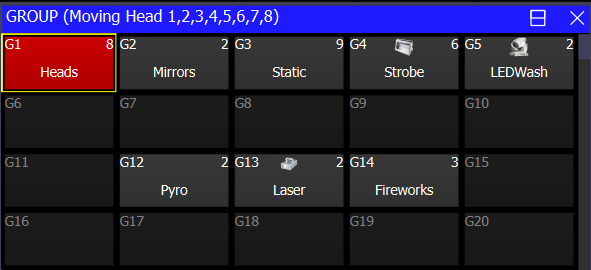
\includegraphics[width=\linewidth]{slika 6-9.png}
	\caption{Grupe uređaja}
	\label{fig:slika 6-9}
\end{figure}

Primjerice, odabirom grupe \emph{Heads} svim pokretnim glavama na svoj prvi kanal (kanal za boju) pošalje se vrijednost 45, na treći kanal (kanal za intenzitet) pošalje se vrijednost 255 te na sedmi i deveti kanal pošalje se vrijednost 128 (kanali za nagib i pomicanje) što rezultira upravljanjem pokretnim glavama u Unreal Engineu kao na slici \ref{fig:slika 6-10}.

\begin{figure}[htp]
	\centering
	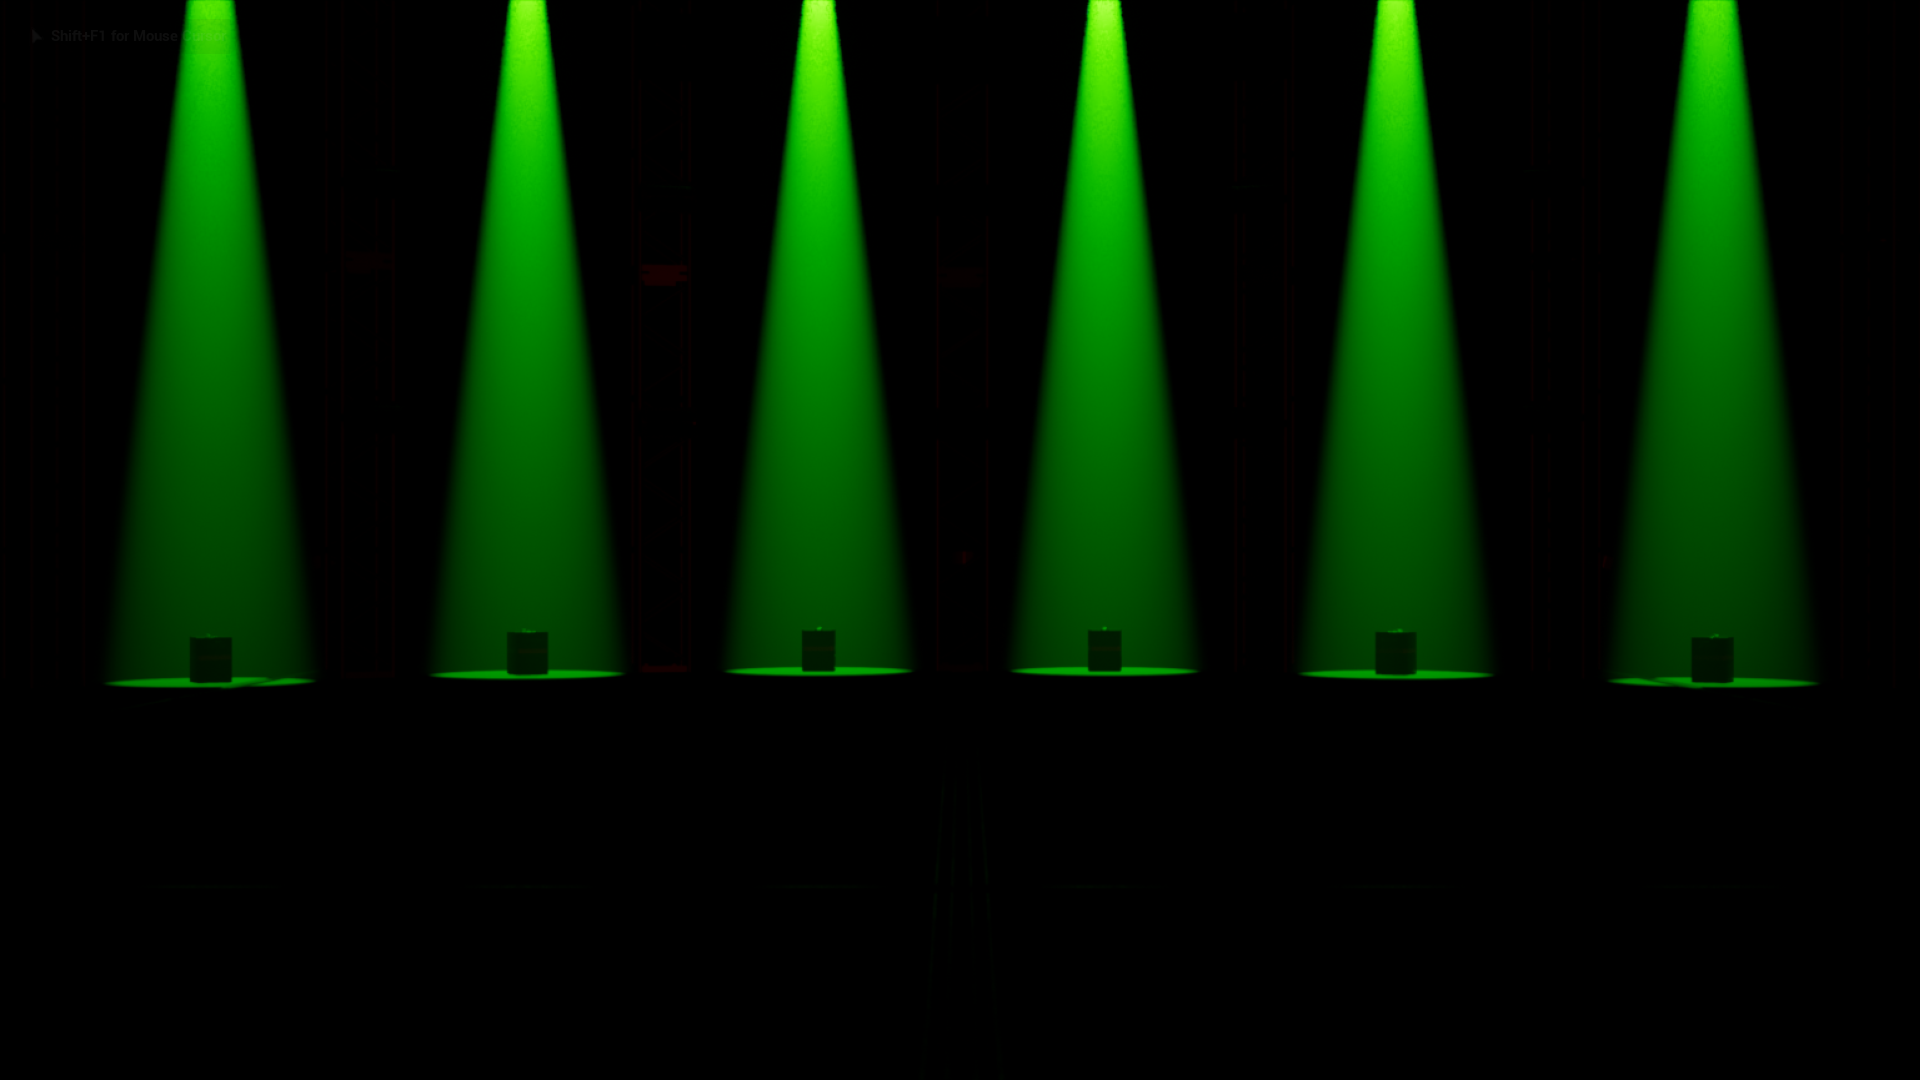
\includegraphics[width=\linewidth]{slika 6-10.png}
	\caption{Upravljanje pokretnim glavama}
	\label{fig:slika 6-10}
\end{figure}

Drugi primjer, odabirom grupe \emph{Pyro} te slanjem vrijednosti 128 rezultira paljenem pirotehničkih efekata (slika \ref{fig:slika 6-11}). Na ovaj način se može upravljati cijelom setom u stvarnom vremenu.

\begin{figure}[htp]
	\centering
	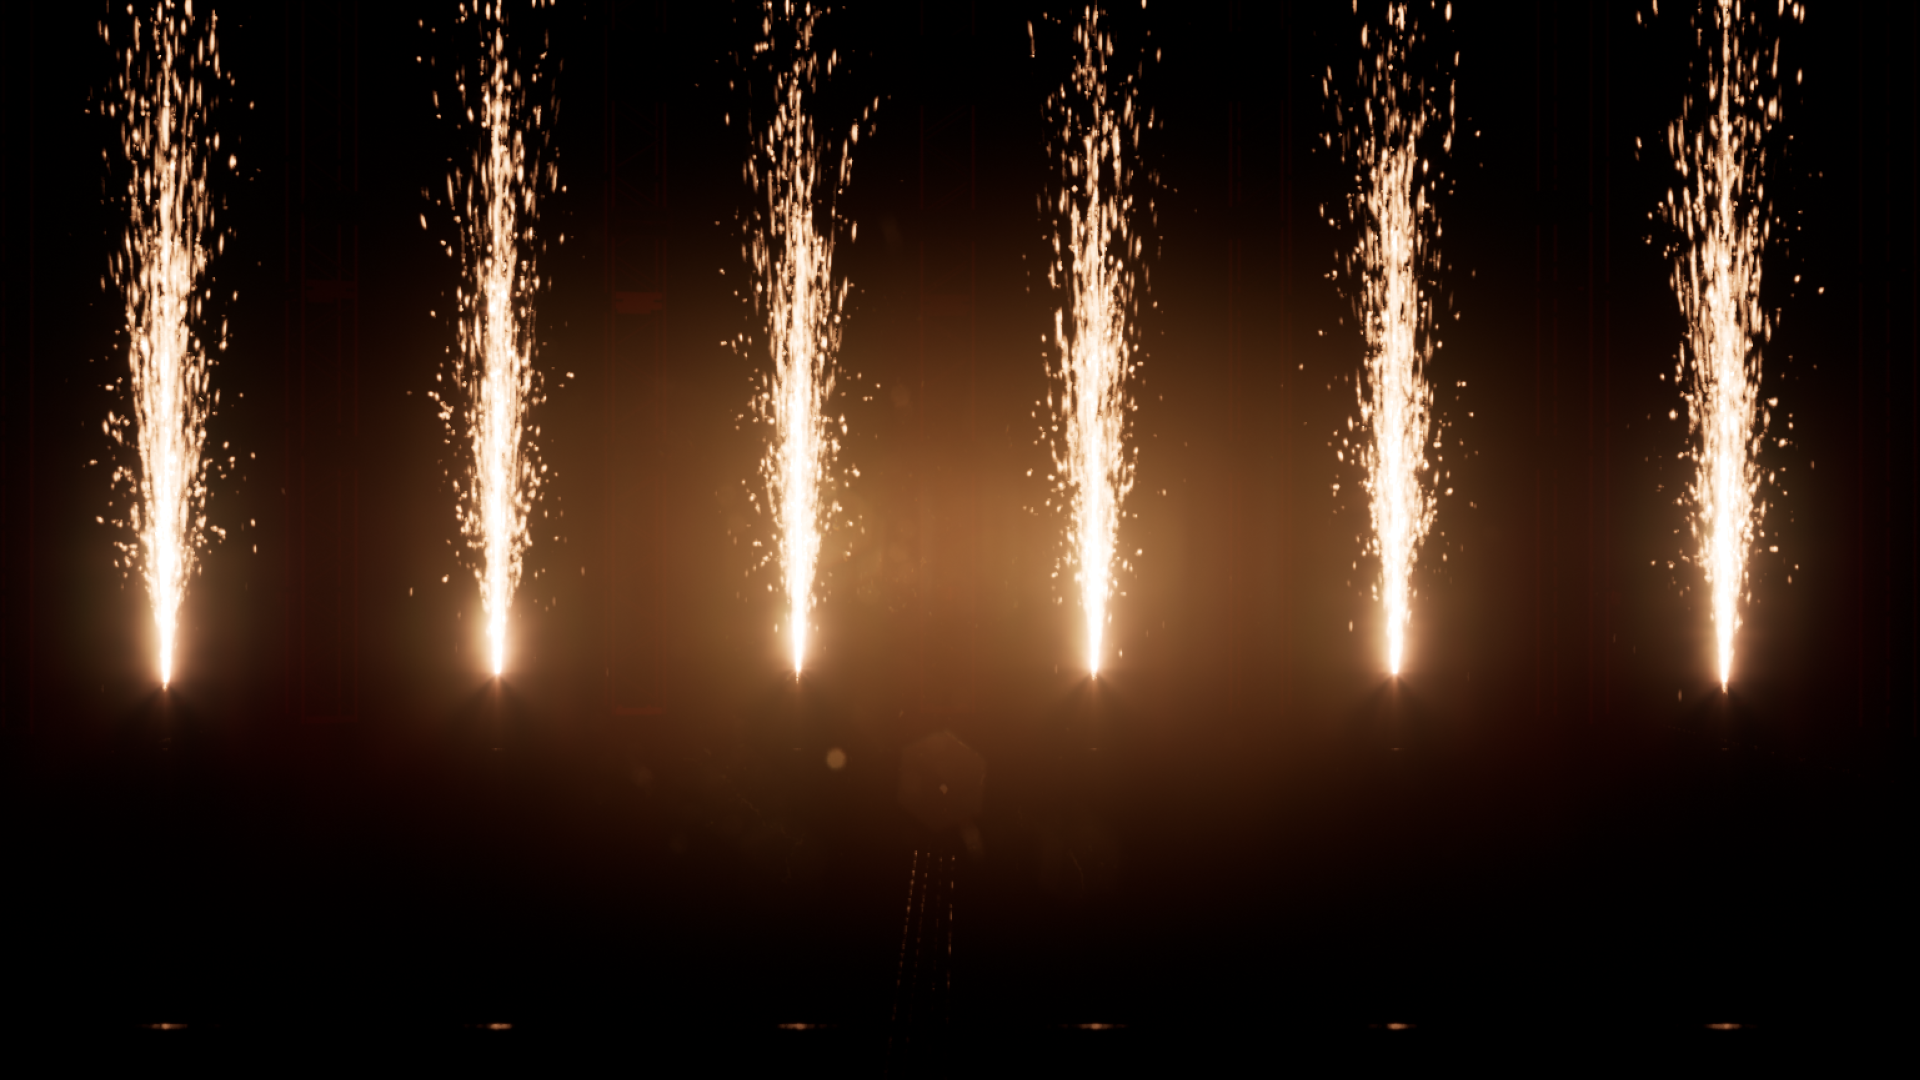
\includegraphics[width=\linewidth]{slika 6-11.png}
	\caption{Paljenje pirotehnike}
	\label{fig:slika 6-11}
\end{figure}

\pagebreak

\subsection{Korištenje sekvencera}

\chapter{Integracija s prototipom}
1\pagebreak

2\pagebreak

3\pagebreak

4\pagebreak
\chapter{Rezultati}
1\pagebreak

2\pagebreak
\chapter{Zaključak}

\raggedright
\bibliography{literatura}
\bibliographystyle{fer}

\begin{sazetak}
Sažetak na hrvatskom jeziku.

\kljucnerijeci{Ključne riječi, odvojene zarezima.}
\end{sazetak}

\pagebreak

\engtitle{CONNECTING VIRTUAL AND REAL LIGHTING USING THE UNREAL SYSTEM}
\begin{abstract}
Abstract.

\keywords{Keywords.}
\end{abstract}

\end{document}